\documentclass[onecolumn]{IEEEtran}
\IEEEoverridecommandlockouts
% The preceding line is only needed to identify funding in the first footnote. If that is unneeded, please comment it out.
\usepackage{cite}
\usepackage{hhline}
\usepackage[most]{tcolorbox}
\usepackage{lineno}
\usepackage{amsmath,amssymb,amsfonts, amsthm}
\usepackage{enumitem}
\usepackage{placeins}
\usepackage{hyperref}
\usepackage{algorithmic}
\usepackage{ltablex}
\usepackage{graphicx}
\usepackage{lipsum}
\usepackage{textcomp}
\usepackage{xcolor}
\usepackage{tikz}
\usepackage{subcaption}

\def\BibTeX{{\rm B\kern-.05em{\sc i\kern-.025em b}\kern-.08em
    T\kern-.1667em\lower.7ex\hbox{E}\kern-.125emX}}

\tcbuselibrary{theorems}
\newtcbtheorem[auto counter, number within=section]{definitionbox}{Definition}{
  colback=gray!5!white,
  colframe=black!60,
  coltitle=black,
  fonttitle=\bfseries,
  boxrule=0.3mm,
  arc=1mm,
  left=1mm,
  right=1mm,
  top=1mm,
  bottom=1mm,
  enhanced,
  sharp corners=south,
  attach boxed title to top left={xshift=0.5cm, yshift=-2mm},
  boxed title style={colback=white, boxrule=0pt},
}{def}

\newtcbtheorem[auto counter, number within=section]{theorembox}{theorem}{
  colback=gray!5!white,
  colframe=black!60,
  coltitle=black,
  fonttitle=\bfseries,
  boxrule=0.3mm,
  arc=1mm,
  left=1mm,
  right=1mm,
  top=1mm,
  bottom=1mm,
  enhanced,
  sharp corners=south,
  attach boxed title to top left={xshift=0.5cm, yshift=-2mm},
  boxed title style={colback=white, boxrule=0pt},
}{thm}

\newtcbtheorem[auto counter, number within=section]{conjecturebox}{Conjecture}{
  colback=gray!5!white,
  colframe=black!60,
  coltitle=black,
  fonttitle=\bfseries,
  boxrule=0.3mm,
  arc=1mm,
  left=1mm,
  right=1mm,
  top=1mm,
  bottom=1mm,
  enhanced,
  sharp corners=south,
  attach boxed title to top left={xshift=0.5cm, yshift=-2mm},
  boxed title style={colback=white, boxrule=0pt},
}{conj}


\newtcbtheorem[auto counter, number within=section]{propositionbox}{Proposition}{
  colback=gray!5!white,
  colframe=black!60,
  coltitle=black,
  fonttitle=\bfseries,
  boxrule=0.3mm,
  arc=1mm,
  left=1mm,
  right=1mm,
  top=1mm,
  bottom=1mm,
  enhanced,
  sharp corners=south,
  attach boxed title to top left={xshift=0.5cm, yshift=-2mm},
  boxed title style={colback=white, boxrule=0pt},
}{prop}



\newtcbtheorem[auto counter, number within=theorem]{lemmabox}{Lemma}{
  colback=gray!5!white,
  colframe=black!60,
  coltitle=black,
  fonttitle=\bfseries,
  boxrule=0.3mm,
  arc=1mm,
  left=1mm,
  right=1mm,
  top=1mm,
  bottom=1mm,
  enhanced,
  sharp corners=south,
  attach boxed title to top left={xshift=0.5cm, yshift=-2mm},
  boxed title style={colback=white, boxrule=0pt},
}{lem}

\newtcbtheorem[auto counter, number within=section]{claimbox}{Claim}{
  colback=gray!5!white,
  colframe=black!60,
  coltitle=black,
  fonttitle=\bfseries,
  boxrule=0.3mm,
  arc=1mm,
  left=1mm,
  right=1mm,
  top=1mm,
  bottom=1mm,
  enhanced,
  sharp corners=south,
  attach boxed title to top left={xshift=0.5cm, yshift=-2mm},
  boxed title style={colback=white, boxrule=0pt},
}{clm}


\newtheorem{theorem}{Theorem}[section]
\newtheorem{conjecture}[theorem]{Conjecture}
\newtheorem{proposition}[theorem]{Proposition}
\newtheorem{lemma}[theorem]{Lemma}
\newtheorem{claim}[theorem]{Claim}
\newtheorem{corollary}{Corollary}[theorem]
\newtheorem{definition}{Definition}[section]

\newcommand{\scn}[1]{\textnormal{\textsc{#1}}}
\newcolumntype{Y}{>{\centering\arraybackslash}X}

\begin{document}

\title{Counting Problem of \textit{PureCircuit}}

\author{\IEEEauthorblockN{Christos Demetriou}
\IEEEauthorblockA{\textit{Department of Computer Science} \\
\textit{University of Warwick}\\
Coventry, UK \\
u2018918@live.warwick.ac.uk, u2018918}}

\maketitle

\begin{abstract}
In the world of combinatronics, one often looks for the combinatronic interpretation between numbers.
Recently, through the works of Igor Pak and other researchers, people have decided
to combine the worlds of counting complexity theory with combinatronics to give formal
definition to this idea \cite{ikenmeyer_WhatWhatNot_2022, ikenmeyer_PositivitySymmetricGroup_2024, pak_WhatCombinatorialInterpretation_2022}. 
Our project focuses on analysing the combinatorial properties of $\textsc{PPAD} -1$ using
the \textsc{PureCircuit} problem as well as developing a visualisation tool for it. In this report, we give a progress report as to the work that 
we have done as well as talk about notable results such as parsimonious reductions between Sperner problems to
\textsc{PureCircuit} up to some constant bound.




\end{abstract}

\section{Introduction}
Combinatronics has been a field of study in mathematics that primarily focuses on
the notion of counting objects with certain properties. Over time, this notion
has shifted, especially in the subfield of algebraic combinatorics, where
there is no clear notion of the object that we are counting,
and the numbers express something more abstract \cite{pak_WhatCombinatorialInterpretation_2022}.
In recent years, there has been a revolutionary
initiative in the field of combinatronics to assign combinatorial interpretations to such numbers.
Being able to find such definitions or interpretations is very important
as it allows us to utilise tools from combinatorics to understand
and reveal hidden structures and properties \cite{pak_WhatCombinatorialInterpretation_2022}. 
Moreover, there are several problems or numbers such as \textit{Kronecker coefficients} \cite{makar_AnalysisKroneckerProduct_1949},
whose combinatorial interpretation, would lead to groundbreaking breakthroughs such as a step closer to the resolution of the $\textit{P} \neq \textit{NP}$
conjecture \cite{ikenmeyer_WhatWhatNot_2022, ikenmeyer_VanishingKroneckerCoefficients_2017}.


% To formalise that idea, Pak et al. has argued that if a function $f$
% belongs to $\textit{\#P}$, it implies that $f$ has a combinatorial interpretation
% \cite{pak_WhatCombinatorialInterpretation_2022, ikenmeyer_WhatWhatNot_2022}. We invest
In our current work, we focus on extending the work done by
Ikenmeyer et al. \cite{ikenmeyer_WhatWhatNot_2022}, where they focused on the creation of frameworks
that determines whether $f \in^? \textsc{\#P}$, by looking
at the subclasses of $\textsc{\#TFNP - 1}$ problems.
In our work we focus specifically on the complexity class of $\textsc{PPAD}$, under the lens of $\text{PureCircuit}$,
due to circuit-based nature.
We hope to uncover many insights of the $\textsc{\#PureCircuit} -1$ problem 
as well as explore the boundaries of $\textsc{\#PPAD} -1$.

% In their paper, they were able to show that for a subclass of
% problems, also known as $\textit{PPAD} \subseteq \textit{TFNP}$,
% different $\textit{PPAD-complete}$ problems, may or may not have a combinatorial
% interpretation.

\subsection{Research Question}

Our objectives revolve around the conjecture in \ref{conj:ppad-1-hardness}, where
we investigate the boundaries of $\scn{\#PPAD}-1$ with the help of the \textsc{PureCircuit} problem.
\begin{conjecturebox}{$\scn{\#PPAD}-1$ hardness}{ppad-1-hardness}
    Every language in \scn{PPAD} can be parsimoniously reduced up to some polynomial factor, to the
    \textsc{PureCircuit} problem, or more formally:
    $$
    \forall L \in \scn{PPAD}, \exists f \in n^{O(1)}: 
    \scn{\#L} \subseteq^f \scn{\#PureCircuit}
    $$
\end{conjecturebox}




\subsection{Project objectives}

To tackle our research question, we propose the following list of objectives. 
These objectives outline a series of reductions between problems that were identified as necessary,
as explained in paragraph \ref{par:count-ppad}.
We hope that by completing these milestones, we will be able to answer our research question.

\begin{enumerate}[label*=R.\arabic*)]
    \item Find a parsimonious reduction from the $\textsc{EndOfLine}$ to $\textsc{PureCircuit}$.
    \item Demonstrate that $\textsc{\#PureCircuit}- 1 \not\subseteq \textsc{\#P}$ either by:
        \begin{enumerate}
            \item Showing that $\textsc{\#SourceOrExcess(k,1)} \subseteq \textsc{\#PureCircuit}$ for some $k \in \mathbb{N}_{\geq 2}$
            \item Showing that $\textsc{\#SourceOrExcess(k,1)} \subseteq \textsc{\#nD-StrongSperner}$ for some $k,n \in \mathbb{N}_{\geq 2}$ 
        \end{enumerate}
    \item Prove or disprove the following:
\[
\forall n \in \mathbb{N}_{\geq 2}, \exists c \in \mathbb{N}:  \scn{\#SourceOrExcess}(n, 1) \subseteq^c \scn{\#PureCircuit}
\]

\end{enumerate}

In addition to expanding the theory of $\textsc{\#PPAD} -1$, we aim to build
a visualisation tool for $\textsc{PureCircuit}$ instances. This tool
will allow us to visualise circuits as well as investigate the behaviour
of $\textsc{PureCircuit}$ for controlled cases. More formally,
we have the following milestones:

\begin{enumerate}[label=S.\arabic*)]
    \item Visualise and verify a \textsc{PureCircuit} instance.
    \item Generate a solution for given a \textsc{PureCircuit} instance.
    \item Count the number of solutions of a \textsc{PureCircuit} instance.
\end{enumerate}

We will compile the rest of the report, based on our current findings, how we altered our previous objectives 
and general reflections. Moreover we will give a brief summary as to the subsequent steps
and how plan to achieve the remaining milestones.


%
% Below we will present our main list of findings up to this point:
%
% \begin{theorem}[ND-Brouwer to PureCircuit]
%     Given $f(x) \triangleq 20$
%     $$
%     \scn{\#Brouwer}^{f_3} \subset^f \scn{\#PureCircuit}
%     $$
% \end{theorem}
%
% \begin{corollary}
%     For any $d \in \mathbb{N}_{\geq 2}$, we can define $f(\cdot) = \sum_{i = 1}^{d -1}  \binom{d}{i} 2^i$
%     such that:
%     $$
%     \scn{\#Brouwer}^{d} \subset^f \scn{\#PureCircuit}
%     $$ 
% \end{corollary}
%
%
%
% \begin{theorem}
%     For any $d \in \mathbb{N}_{\geq 2}$, we can define $f(\cdot) = 5$
%     such that:
%     $$
%     \scn{\#Brouwer}^d \subseteq^f \scn{\#PureCircuit}
%     $$ 
% \end{theorem}
%
%
% Throughout our search, we stumbled upon
% various variants of the problem as well as reductions and claims from other
% subclasses of PPAD or Hazard-Free logic
%
% \begin{proposition}
%     Weaker variants of PureCircuit can result to parsimonious reductions to the EndOfLine problem
%     as such:
%     \begin{gather*}
%         \scn{\#AcyclicBPureCircuit} \subseteq \scn{\#EndOfLine} \\
%         \scn{\#PermutationFreeBPureCircuit} \subseteq \scn{\#EndOfLine}
%     \end{gather*}
% \end{proposition}
%
%
% In addition, we were able to show that for different promise problems,
% we can find reductions to the PureCircuit problem
% %
% \begin{proposition}
%     $$
%         \scn{\#PUnsatHazard} \subseteq  \scn{\#PureCircuit}
%     $$
% \end{proposition}
%
% Lastly we introduce the following proposition
% \begin{proposition}
%     Given function $F: \mathbb{T}^n \to \mathbb{T}^n$
%     where $\mathbb{T} \triangleq \{0, 1, \bot\}$ and $F$ is a \textbf{natural}
%     function:
% $$
% \exists x^\star \in \mathbb{T}^n: F(x^\star) = x^\star
% $$
% \end{proposition}
% %
%
% The idea above is based on the Tarski Fixed point theorem.
% Using fixed points with the Kleene logic set, has been used in the past
% by Kozer as seen in his book \cite{kozen2006theory}, but we
% are extending such ideas to any possible functions or gates
% that use monotone gates. Doing that allows us to make the following observation.
%
% \begin{proposition}
%     $$
%     \scn{\#HazardTarski} \subseteq \scn{\#PureCircuit}
%     $$
% \end{proposition}
%


\section{Preliminaries and Background review}
% LTeX: enabled=true

\subsection{Important Notation}

To avoid ambiguity, we introduce the following notation conventions used throughout the paper.
For any $n \in \mathbb{N}$, we write $[n] \triangleq \{1, \ldots, n\}$  and $[n]_0 \triangleq [n] \cup \{0\}$. 
We define the Boolean domain as $\mathbb{B} \triangleq \{0, 1\}$ and
three value domain $\mathbb{T} \triangleq \{0, 1, \bot\}$.


\subsection{Background overview}


\subsubsection{Counting Complexity and Combinatorial Interpretations}

Counting complexity looks into complexity of counting solutions using notions
such as $\textbf{\#P}$.
$\textbf{\#P}$ was created by \cite{valiant_ComplexityComputingPermanent_1979},
to demonstrate the difficulty of counting the number of solutions to a problem,
even they are polynomially verifiable.

\begin{definitionbox}{$\textsc{\#P}$ Complexity Clas \cite{valiant_ComplexityComputingPermanent_1979}}{sharpp-class}
    $\textbf{\#P}$ is a class of functions $f: \mathbb{B}^* \to \mathbb{N}$
    such that: there
    exists a polynomial-time deterministic TM $M$, and
    $p : \mathbb{N} \to \mathbb{N}$ such that $p \in n^{O(1)}$, we have:
    $$
    f(w) = \Big|\Big\{v \in \mathbb{B}^{p(|w|)} \mid M(w, v) =1 \Big\}\Big|
    $$
\end{definitionbox}


As we can see, $\textbf{\#P}$ allows us to define a set of objects,
whose cardinality equals $f(w)$. The reason for choosing
$\textbf{\#P}$ to define combinatorial interpretations is \cite{ikenmeyer_PositivitySymmetricGroup_2024}: 

\begin{enumerate}
    \item By polynomially bounding words, we avoid cases such as: $f(w) = |\{1, \hdots, f(w)\}|$.
    \item Work wtih $f(\cdot)$, even if its direct computation is hard.
\end{enumerate}


The current framework was used in several papers such as
\cite{ikenmeyer_WhatWhatNot_2022} and \cite{ikenmeyer_PositivitySymmetricGroup_2024}
where they were able to use tools from complexity theory to show that
many structures do or do not have a combinatorial interpretation.
Lastly we introduce the idea of correlating two counting problems with the help of
\textit{parsimonious reductions} \ref{def:pars-reduction}.


\begin{definitionbox}{Parsimonious reductions}{pars-reduction}
    Let $R, R'$ be search problems and let $f$ be a reduction of
    $S_R = \{x \mid R(x) \neq \emptyset \}$ to $S_{R'} = \{x \mid R'(x) \neq \emptyset \}$.
    We say $f$ is \textbf{parsimonious} if:
    $$
    \forall x \in S_R : |R(x)| = |R'(f(x))|
    $$ 
\end{definitionbox}

Below we are introducing a variant of parimonious reductions that allows
for one-to-many reductions. 
\begin{definitionbox}{Poly-Function Bounded Parsimonious Reductions}{func-pars}
    Given two counting problems $A, B : \mathbb{B}* \to \mathbb{N}$
    and a function $f : \mathbb{B}^{*} \to \mathbb{N}$ such that $f \in n^{O(1)}$, we
    say that:
    $$
    A \subseteq^f B
    $$
    If for input $w \in \mathbb{B}^*$, if $a$ represent the number of solutions
    for problem $A$ and $b$ the number of solutions for problem $B$, we have:
    $$
    a \leq b \leq f(|w|) \cdot a
    $$
    If $\forall x : f(x) = c$ for $c \in \mathbb{N}$ then we will just say 
    $$
    A \subseteq^c B
    $$
\end{definitionbox}

\subsubsection{Total Search Problems and PPAD}
We give a brief overview of \textbf{TFNP} and \textbf{PPAD}.


\begin{definitionbox}{Search Problems and Total Search Problems}{search-problems}
    \textbf{Search problems} can be defined as relations $R \subseteq \mathbb{B}^* \times \mathbb{B}^*$,
    where given $x \in \mathbb{B}^*$, we want to find $y \in \mathbb{B}^*$  such that $x Ry$.

    \textbf{Total Search problems} are search problems such that:
    $$
    \forall x \in \mathbb{B}^*, \exists y \in \mathbb{B}^* : xRy
    $$
\end{definitionbox}


\begin{definitionbox}{$\scn{FNP}$ and $\scn{TFNP}$}{fnp-tfnp}
    \textbf{FNP} are \textit{search problems} such that there exists poly-time TM $M: \mathbb{B}^* \to \mathbb{B}$
    and a poly function $p : \mathbb{N} \to \mathbb{N}$ such that:
    $$
    \forall x \in \mathbb{B}^*, y \in \mathbb{B}^{p(|x|)}: xRy \iff M(x,y) = 1
    $$
    Lastly $\textbf{TFNP} = \{L \in \textbf{FNP} \mid L \text{ is total}\}$
\end{definitionbox}

%
% \begin{definitionbox}{Levin Reductions}{levin-red}
%     Given a pair of search problems $R_A, R_B$, a pair of
%     computable time functions $(f,g)$ is called a Levin reduction from $R_A \to R_B$
%     \begin{gather*}
%         S_R \triangleq \{x \mid \exists y : xRy  \}\\
%         R(x) \triangleq \{y \mid x Ry \} \\
%         \forall x \in S_{R_A}, y_b \in R(f(x)):  (x , g(x, y_b)) \in R_A
%     \end{gather*}
% \end{definitionbox}


Our current work focuses on a specific subclass of $\textbf{TFNP}$ problems
which is defined as follows:

\begin{minipage}{0.55\linewidth}
\begin{definitionbox}{\textit{EndOfLine} problem \cite{papadimitriou_ComplexityParityArgument_1994}}{eol-ppad}
    Given circuits $S, P \in \mathbb{B}^n \to \mathbb{B}^n$ such that $S,P \in n^{O(1)}$
    we define a directed graph $G = (V,E)$, such that $V= \mathbb{B}^n$ and $E$ defined as:
    $$
    E = \{(x,y) \in V^2: S(x) = y \wedge P(y) = x\}
    $$
    We define source or sinks $\forall v \in V: \textit{deg}(v) = (0,1)$ or
    $\textit{deg}(v) = (1,0)$, respectively. 
    We also syntactially ensure that the $0^n$ node is always a source, meaning
    $S(P(0^n) \neq 0 \wedge P(S(0^n)) = 0^n$.
    A node $v \in V$ is a solution if and only if $\textit{deg}(v)$ is either
    $(0,1)$  or $(1,0)$.
\end{definitionbox}
\end{minipage}
\begin{minipage}{0.45\linewidth}
    \centering
    \includegraphics[width=0.7\linewidth]{assets/eol-subgraphs.png}
    \captionof{figure}{Types of subgraphs in \textsc{EndOfLine}}\label{fig:eol-subgraphs}
\end{minipage}

\vspace{0.2cm}

An illustrative example of an instance can be seen in the figure \ref{fig:eol-subgraphs}. 
Using the \textsc{EndOfLine} problem, we define the
\textsc{PPAD} complexity class \ref{def:ppad-complexity-class}


\begin{definitionbox}{\textsc{PPAD} complexity class \cite{papadimitriou_ComplexityParityArgument_1994}}{ppad-complexity-class}
    \textsc{PPAD} is defined as the set of search problems that
    are reducible to the \scn{EndOfLine} problem \ref{def:eol-ppad}.
\end{definitionbox}

\textbf{PPAD} has been created by Papadimitriou \cite{papadimitriou_ComplexityParityArgument_1994}
to demonstrate a subset of problems in \textbf{NP} that are guaranteed to have
a solution but can be very difficult to find. In the next section
we will introduce the relevant of \textsc{PPAD} problems.

\paragraph{The PureCircuit problem}
\label{par:pure-circ-def}

The  \textsc{PureCircuit} was created by Deligkas et al. \cite{deligkas_PureCircuitTightInapproximability_2024}
to demonstrate the hardness of approximating \textsc{PPAD} problems.
it uses kleene-logic based circuits and with continuity of arguments, they demonstrated \textsc{PPAD-completeness}.

\begin{definitionbox}{\textsc{PureCiruit} Problem Definition \cite{deligkas_PureCircuitTightInapproximability_2024}}{purecircuit-def}
An instance of \textit{PureCircuit} is given by vertex set $V= [n]$ and gate set $G$ such that
$\forall g \in G: g=(T,u,v,w)$ where $u,v,w \in V$ and $T \in \{\text{NOR}, \text{Purify}\}$.
Each gate is interpreted as:
\begin{enumerate}
    \item \textit{NOR}: Takes as input $u,v$ and outputs $w$
    \item \textit{Purify}: Takes as input $u$ and outputs $v,w$
\end{enumerate}
And each vertex is ensured to have $\text{in-deg}(v) \leq 1$.
A solution to input instance $(V,G)$ is denoted as an assignment $\mathbf{x} : V \to \{0, \bot, 1\}$
such that for all nodes we have:
\begin{enumerate}
    \item if $v$ is the output of a $(\textit{NOR}, u,v,w)$ gate:
       \begin{gather*}
            \mathbf{x}[u] = \mathbf{x}[v] = 0 \implies \mathbf{x}[w] = 1\\
            (\mathbf{x}[u] =1 \vee \mathbf{x}[v] =1) \implies \mathbf{x}[w] = 0 \\
            \text{otherwise} \implies \bot
        \end{gather*}

    \item \textit{Purify}: 
       \begin{gather*}
           \forall b \in \mathbb{B}: \mathbf{x}[u] = b \implies \mathbf{x}[v] = b \wedge \mathbf{x}[w] =  b\\
           \mathbf{x}[u] = \bot \implies \{\mathbf{x}[v] \cup \mathbf{x}[w] \} \cap \mathbb{B}\neq \emptyset
        \end{gather*}
\end{enumerate}
\end{definitionbox}

The definition of \textsc{PureCircuit} that we will be using for the standard set of gates
$\{\wedge, \vee, \neg\}$, is based Kleene's three-valued strong logic of indeterminancy
which extends the traditional $\mathbb{B}$ logic \cite{kleene_IntroductionMetamathematics_2009}.
Their behaviour can be described in the tables shown in \ref{tab:three-val-logic}
In addition to that, we will make use of the \textit{Copy} gate which we can define as $\textit{Copy}(x) = \neg (\neg x)$.
This allows our circuits to be robust and easier to work with.

\begin{table}[h!]
    \centering
    \subfloat[\texttt{not} gate]{
    \begin{tabular}{c|c}
\texttt{not} & \textbf{} \\
\hline
0 & 1 \\
$\bot$ & $\bot$ \\
1 & 0 \\
\end{tabular}
}
\subfloat[\texttt{and} gate]{
\begin{tabular}{c|ccc}
\texttt{and} & 0 & $\bot$ & 1 \\
\hline
0    & 0 & 0 & 0 \\
$\bot$ & 0 & $\bot$ & $\bot$ \\
1    & 0 & $\bot$ & 1 \\
\end{tabular}
} \quad
\subfloat[\texttt{or} gate]{
\begin{tabular}{c|ccc}
\texttt{or} & 0 & $\bot$ & 1 \\
\hline
0    & 0     & $\bot$ & 1 \\
$\bot$ & $\bot$  & $\bot$ & 1 \\
1    & 1 & 1 & 1 \\
\end{tabular}
}

    \caption{Three-valued logic \cite{kleene_IntroductionMetamathematics_2009}}\label{tab:three-val-logic}
\end{table}




For the \textit{Purify} gate,
Deligkas et al. showed that the only solutions that are essential for \textit{Purify}
are $\{(0,\bot), (\bot,1), (0,1)\}$ with the help of continuity arguments \cite{deligkas_PureCircuitTightInapproximability_2024}.
Adding more solutions does not change the complexity as he showed in the original variant of the problem.
We acknowledge that the solution set will be different from the original one but,
one can observe that  $\textsc{\#PureCircuit-simplified} \subseteq \textsc{\#PureCircuit}$,
and therefore any proposition or argument of the sort:
$\textsc{\#A} \subseteq \textsc{\#PureCircuit-simplified} \implies \textsc{\#A} \subseteq \textsc{\#PureCircuit}$.
For the purposes of the report, any solution change will be made explicit
and we will refer to all such simplified variants as $\textsc{\#PureCircuit}$ to avoid
confusion. 



\begin{definitionbox}{\textsc{SourceOrExcess} problem}{source-or-excess}
    We define as $\textit{SourceOrExcess}(k,1)$ for $k \in \mathbb{N}_{\geq 2}$
    the search problem as such: Given a poly-sized successor circuit $S : \mathbb{B}^n$
    and a set of predecssor poly-sized circuits $\{P_i\}_{i \in [k]}$, we define
    the graph $G = (V,E)$ such that, $V = \mathbb{B}^n$ and $E$ as:
    $$
    \forall x, y \in V: (x,y) \in E \iff (S(x) = y) \wedge \bigvee_{i \in [k]} P_i(y) = x
    $$
    We ensure that $0^n$ is as sink, meaning $\text{deg}(0^n) = (0,1)$.
    A valid solution is a vertex $v$ such that $\textit{in-deg}(v) \neq \textit{out-deg}(v)$
\end{definitionbox}

\paragraph{Sperner problems}

Below we will refer to the notion of Sperner problems which involve
the idea of using the topology of a problem and a colouring scheme to ensure
that a substructure is panchromatic. There two variants of colouring scheme
that are used: one of them will be referred to as the \textbf{linear} colouring
where for dimension $d$, assign $d+1$ distinct colours to each point \cite{daskalakis_ComplexityComputingNash_2006, chen_Complexity2DDiscrete_2009}.
Below we will refer to \textbf{bipolar} colouring, which has been used grid-like topologies of the Sperner property
\cite{chen_SettlingComplexityComputing_2009, deligkas_PureCircuitTightInapproximability_2024, daskalakis_ComplexityConstrainedMinmax_2021}.
It has to be noted that these are not their official names, but we have decided
to use this naming scheme for clarity.



\begin{definitionbox}{Bipolar colouring}{bipolar-colouring}
    Given dimension $d$, we refer to the bipolar colouring $C$ of a point $v \in S^d$
    where $S$ is some arbitrary set in $d$ dimensionality the following:
    $$
    \forall j \in [d]: [C(v)]_j \in \{-1,1\}
    $$
    Essentially a point is a associate with a $d$ dimensionaly binary vector.
    We say that a set of points $A \subseteq S^d$ \textbf{cover all the labels} if:
    $$
        \forall i \in [d], \ell \in \{-1, +1\}, \exists x \in A: [\lambda(x)]_{i} = \ell
    $$
\end{definitionbox}



\begin{definitionbox}{\textsc{StrongSperner} problem}{strong-sperner}
    \textbf{Input}: A boolean circuit that computes a bipolar labelling $\lambda: [M]^N \to \{-1, 1\}^N$ \ref{def:bipolar-colouring}
    satisfying the following boundary conditions $\forall i \in [N]$:
    \begin{itemize}
        \item if $x_i = 1 \implies [\lambda(x)]_i = +1$
        \item if $x_i = M \implies [\lambda(x)]_i = -1$
    \end{itemize}
    \textbf{Output}: A set of points $\{x^{(i)}\}_{i \in [N]} \subseteq [M]^{[N]}$, such that:
    \begin{itemize}
        \item \textit{Closessness condition}: $\forall i,j \in [N]: \|x^{(i)} - x^{(j)}\|_{\infty} \leq 1$
        \item \textit{Covers all labels} as defined in \ref{def:bipolar-colouring}
    \end{itemize}
\end{definitionbox}

The above is a generalised variant of the tradtional Sperner problem to
a grid of dimensions $N$ and width of $M$. 
Throughout literature the same variants of the problem or specifications
have been defined using sperner or discrete brouwer \cite{chen_SettlingComplexityComputing_2009, chen_Complexity2DDiscrete_2009, daskalakis_ComplexityComputingNash_2006, deligkas_PureCircuitTightInapproximability_2024}.
For the sake of clarity, we will stick to $\textsc{StrongSperner}$.

\begin{definitionbox}{$\scn{nD-StrongSperner}$ problem}{nd-strong-sperner}
    \textbf{Input}: A tuple $(\lambda,0^k)$ of a $\scn{StrongSperner}$ instance but for only $n$ dimensions, such that
    $\lambda : (\mathbb{B}^k)^n \to \{-1, +1\}^n$.\\
    \textbf{Output}: A point $\alpha = (a_1, \hdots, a_n) \in A^n$, where $A=\mathbb{B}^k \setminus \{1^k\}$ such that:
    $$
    \{\alpha + x \mid x \in \mathbb{B}^n\} \text{ cover all the labels \ref{def:bipolar-colouring}}
    $$
    We use $A$ to avoid edge cases. We assume dimensionality $n \geq 2$.
\end{definitionbox}

Chen et al. \cite{chen_SettlingComplexityComputing_2009} demonstrated 
that all $\textsc{nD-StrongSperner}$ are $\textsc{PPAD-complete}$.
We mainly use this to show counting arguments with respect to the
\textsc{EndOfLine} as people have indicated a parsimonious reduction
between $\textsc{2D-StrongSperner}$ 
and $\textsc{3D-StrongSperner}$ to the EndOfLine problem but 
with \textit{linear} colouring. The authors of these papers
use these problems indifferently when talking about the reductions
and therefore we can assume that either colouring will create a correct reduction.

\paragraph{Other PPAD problems} 

We will define several problems in \textsc{PPAD} that are related with our project
and demonstrate the counting complexity of \textsc{PureCircuit}.

\begin{definitionbox}{\textsc{SourceOrExcess} problem}{source-or-excess}
    We define as $\textit{SourceOrExcess}(k,1)$ for $k \in \mathbb{N}_{\geq 2}$
    the search problem as such: Given a poly-sized successor circuit $S : \mathbb{B}^n$
    and a set of predecssor poly-sized circuits $\{P_i\}_{i \in [k]}$, we define
    the graph $G = (V,E)$ such that, $V = \mathbb{B}^n$ and $E$ as:
    $$
    \forall x, y \in V: (x,y) \in E \iff (S(x) = y) \wedge \bigvee_{i \in [k]} P_i(y) = x
    $$
    We ensure that $0^n$ is as sink, meaning $\text{deg}(0^n) = (0,1)$.
    A valid solution is a vertex $v$ such that $\textit{in-deg}(v) \neq \textit{out-deg}(v)$
\end{definitionbox}

Lastly we will introduce \textsc{Tarski} \ref{def:tarski-ppad}, which is a problem in $\textsc{PLS} \cap \textsc{PPAD}$
where $\textsc{PLS}$ is a class of problems based on the idea of local search \cite{johnson_HowEasyLocal_1988}
and uses the Knaster-Tarski fixed point theorem \ref{thm:knaster-tarski}. We will use this problem in later
sections to connect Kleene algebra with \textsc{PPAD}.


\begin{definitionbox}{Monotone functions}{mono-func}
    Given two posets $(L_1, \preceq_{L_1})$ and $(L_2, \preceq_{L_2})$, a function
    $f: L_1 \to L_2$ is \textbf{monotone} if and only if:
    $$
    \forall x,y \in L_1: x \preceq_{L_1} y \implies f(x) \preceq_{L_2} f(y)
    $$
\end{definitionbox}
    

\begin{theorembox}{Knaster Tarski Fixed point theorem\cite{bronislaw_TheoremeFunctionsDensembles_1928, fearnley_FasterAlgorithmFinding_2022}}{knaster-tarski}
    Given a lattice $(L, \wedge, \vee)$ and a \textit{monotone} $f: L \to L$ \ref{def:mono-func}
    $$
    \exists c \in L: f(c) = c
    $$
\end{theorembox}

Using the Tarski theorem, Fearnley et al. \cite{fearnley_FasterAlgorithmFinding_2022}
created a \textsc{TFNP} variant of the problem which finds fixed points or 
identifies points that break the monotone argument. We will be using Tarski 
with Kleene logic to connect the two.
% \begin{definitionbox}{$\scn{Tarski}$ problem definition \cite{fearnley_FasterAlgorithmFinding_2022}}{tarski-ppad}
%     Given a lattice $(L, \wedge, \vee)$, and a \textit{monotone} function $f : L \to L$ 
%     we define solutions to the problem as:
%     \begin{enumerate}
%         \item Find $x \in L: f(x) = x$
%         \item Find $x,y \in L$ such that $x \preceq y$ and $f(x) \not\preceq f(y)$
%     \end{enumerate}
%     We assume that $f$ is described by circuit.
% \end{definitionbox}
%
\paragraph{Counting complexity of PPAD}

The current project looks on the counting complexity of such problems as despite two problems
being \textsc{PPAD-complete}, Ikenmeyer et al. \cite{pak_WhatCombinatorialInterpretation_2022} has showed examples where
their counting difficulty can differ vastly as it can be seen in the figure \ref{fig:ppad-count-hier}.

\begin{figure}[h!]
    \centering
    \includegraphics[width=0.5\textwidth]{assets/chart-plot.png}
    \caption{Hierarchy graph between \textsc{\#PPAD} problems. Figure from \cite{ikenmeyer_WhatWhatNot_2022}}\label{fig:ppad-count-hier}
\end{figure}


\subsubsection{Kleene Logic and Hazard-Free Circuits}

Kleene logic uses the boolean system with an additional \textit{unstable} value \cite{kleene_IntroductionMetamathematics_2009}. 
Study of Kleene logic aided in
the development of robust physical systems \cite{friedrichs_MetastabilityContainingCircuits_2018}, as well as
giving definitions to \textit{Alternative Turing mahcines} \cite{kozen_TheoryComputation_2006}, and
showing correlations complexity of monotone circuits sizes
\cite{eichelberger_HazardDetectionCombinational_1965, ikenmeyer_ComplexityHazardfreeCircuits_2019,ikenmeyer_KarchmerWigdersonGamesHazardfree_2022,  bund_SmallHazardFreeTransducers_2025}. 

Our current report will focus on specific concepts with Kleene logic as \textsc{PureCircuit} instances
use the underlying logic directly. Below we introduce important concepts \cite{mukaidono_BternaryLogicFunction_1972}.

\begin{definitionbox}{Kleene value ordering \cite{mukaidono_BternaryLogicFunction_1972}}{kleene-order}
    The instability ordering for $\leq^u$ is defined as: $\bot \leq^u 0,1$. The $n$-dimensional
    extension of the ordering is:
    $$
    \forall x,y \in \mathbb{T}^n: x \leq^u y \implies \forall j \in [n]: (x_j \in \mathbb{B} \implies x_i = y_i)
    $$
\end{definitionbox}


\begin{definitionbox}{Kleene Resolutions \cite{mukaidono_BternaryLogicFunction_1972, ikenmeyer_ComplexityHazardfreeCircuits_2019}}{kleene-res}
    Given $x \in \mathbb{T}^n$, we define the \textit{resolutions} of $x$, using the following notation:
    $$
    \scn{Res}(x) \triangleq \big\{ y \in \mathbb{B}^n \mid x \leq^u y  \big\}
    $$
\end{definitionbox}

Detecting hazards is a concept that is analysed heavily when talking about Kleene logic.
The idea is ensuring robustness of our circuits, meaning if all resolutions of $x \in \mathbb{T}^n$
give the same value, then we should expect circuit to behave the same way \ref{def:hf-def}.
An example of hazard values can be seen in the figure \ref{fig:hazard-example}.

\begin{definitionbox}{Hazard \cite{ikenmeyer_ComplexityHazardfreeCircuits_2019, eichelberger_HazardDetectionCombinational_1965}}{hf-def}
    A \textit{circuit} $C$, on $n$ inputs has \textbf{hazard} at $x \in \mathbb{T}^n \iff C(x) = \bot$
    and $\exists b \in \mathbb{B}, \forall r \in \scn{Res}(x): C(r) = b$. If such value does not exists
    then we say that $C$ is hazard-free.
\end{definitionbox}

\begin{figure}[h!]
    \centering
    \subfloat[Multiplexer with hazard at $(1,1,\bot)$]{\includegraphics[width=0.3\textwidth]{assets/hazard_circuit.png}}
    \subfloat[Hazard free multiplexer]{\includegraphics[width=0.3\textwidth]{assets/hazard-free-circuit.png}}
    \caption{Hazard circuit and hazard-free circuit. Figure by \cite{ikenmeyer_ComplexityHazardfreeCircuits_2019}}\label{fig:hazard-example}
\end{figure}

\begin{definition}[K-bit Hazard]
    For $k \in \mathbb{N}$ at $x \in \mathbb{T}^n \iff C$  has a \textit{hazard} at $x$ and $\bot$ appears at most $k$ times in $x$
\end{definition}
%
%
%


\section{Current Progress}
\subsection{Theoretical Progress}
\subsubsection{EndOfLine to PureCircuit Constant Parsimonious Reduction}

We will define the necessary prerequisites for the current section:

\begin{definition}[Poly-Function Bounded Parsimonious Reductions]
    Given two counting problems $A, B : \{0,1\}* \to \mathbb{N}$
    and a function $f : {0,1}^{*} \to \mathbb{N}$ such that $f \in n^{O(1)}$, we
    say that:
    $$
    A \subseteq^f B
    $$
    If for input $w \in \{0,1\}^*$, if $a$ represent the number of solutions
    for problem $A$ and $b$ the number of solutions for problem $B$, we have:
    $$
    a \leq b \leq f(|w|) \cdot a
    $$
\end{definition}

\begin{proposition}[EndOfLine to 3D-StrongSperner Parsimonious reduction]
    $$
    \scn{\#EndOfLine} \subseteq \scn{\#3D-StrongSperner}
    $$
\end{proposition}

The above has been shown by %% Insert citation
Our main contribution comes from the following theorem


\begin{theorem}[3D-StrongnSperner to PureCircuit]
    Given $f(\cdot) = 20$, we argue
    $$
    \scn{\#3D-StrongSperner} \subseteq^f \scn{\#PureCircuit}
    $$
    Where $\scn{3D-StrongSperner}$ is represented as a tuple $(\lambda, 0^n)$
    where $n$ corresponds to grid size of $2^n$.
\end{theorem}

To show the above holds true we will first show the construction and
prove its correctness.
To simplify the counting argument, we modify a solution of $\textsc{3D-StrongSperner}$
as such: Assuming $S \subseteq \{0,1\}^n$ is the set of all solutions, such that we define $S$ as such:

\begin{align*}
    S &\triangleq \Big\{(i,j,k) \in (\{0,1\}^{n})^3 \mid  \\
      &\{\lambda(i + x_1, j + x_2, k + x_3) \mid x \in \{0,1\}^3 \}\Big\} \text{ covers all labels}
\end{align*}

We will create $\Lambda: (\{0,1\}^{(n+1)})^3 \to \{-1, +1\}^3$ such that
 
$$
    \forall (i,j,k) \in (\{0,1\}^{(n+1)})^3: \Lambda(i,j,k) \triangleq 
\lambda\left( \left\lfloor  \frac{{i+1}}{2}  \right\rfloor, \left\lfloor  \frac{{j+1}}{2} \right\rfloor, \left\lfloor  \frac{{k+1}}{2} \right\rfloor \right)  \\
$$

Conversely we can say that we map from our original domain to our new domain as such

$$
\forall  x \in \{ 0,1 \}^{3n}, i \subseteq \{ 0,1,2 \}: \lambda(x_{-i}, x_{i}) \to \Lambda(2x_{i}, 2x_{-i} -1)
$$

The above transformation can be visualised using the following figure

\begin{figure}[h!]
    \centering
    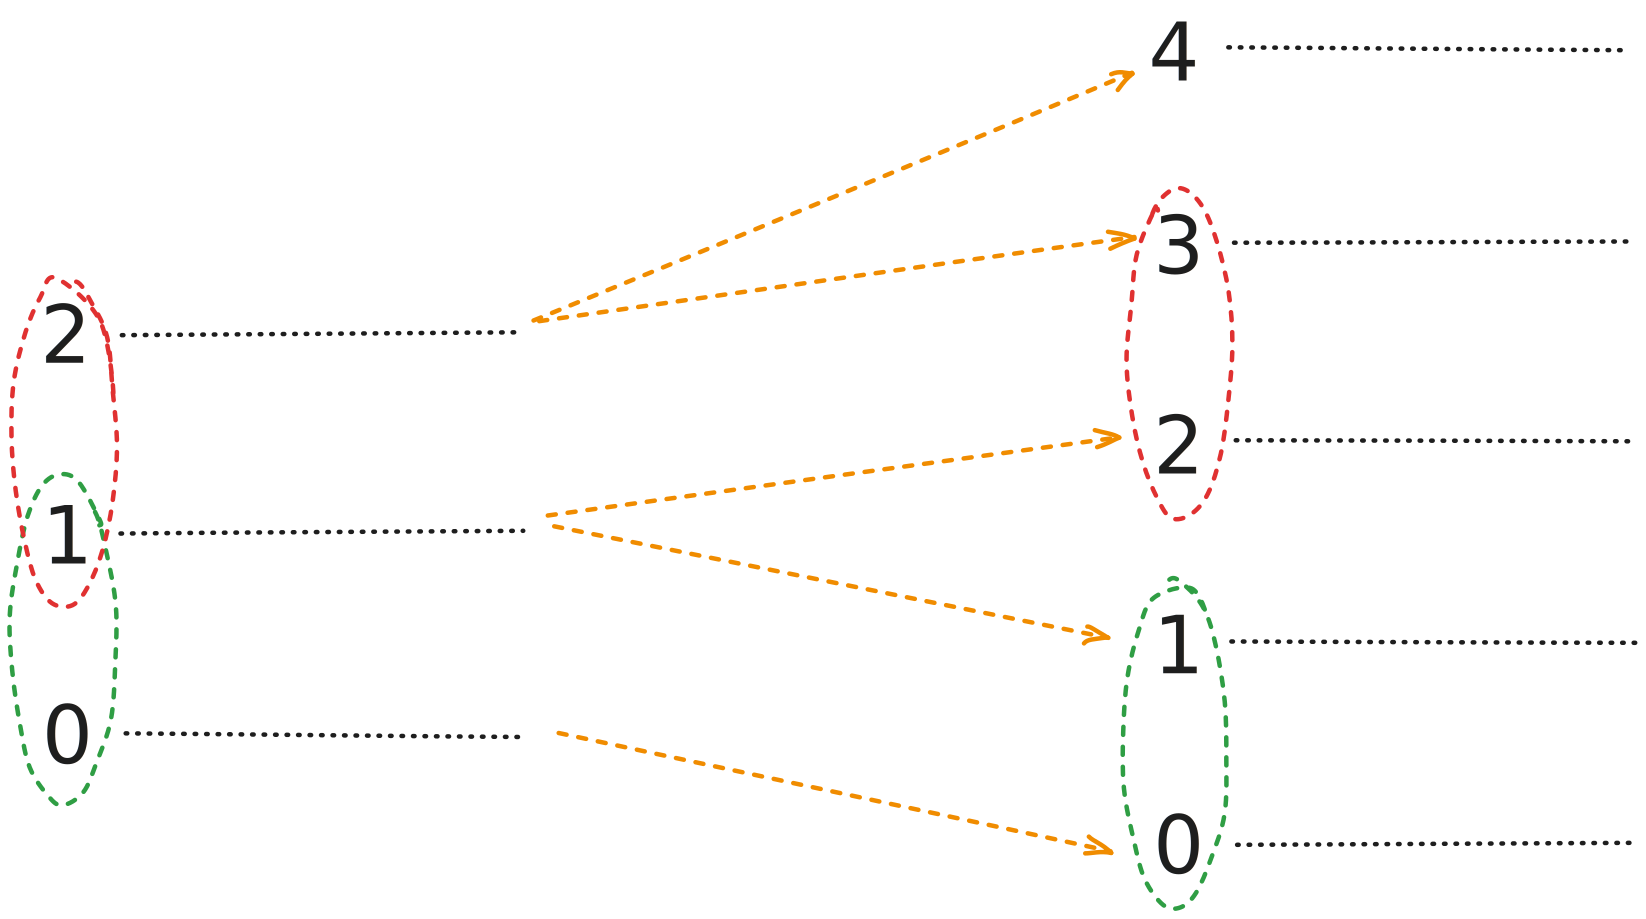
\includegraphics[width=0.5\textwidth]{assets/1751381227.png}
    \caption{The current figure allows depicts how solutions or pairs of solutions are mapped. For example for cube starting at 
        $i = 0$ and $i = 1$, we now just have to look at $i = 0$ and $i = 2$.}
    \label{fig:main-proof:set_mapping}
\end{figure}


\begin{claim}[Transformation claim]
    \label{clm:main-proof:trans-claim}
    We claim that $|S_{\text{even}}| = |S|$ where $S_{\text{even}}$  is defined as:
    $$
S_{\text{even}} \triangleq
   \Big\{(i0,j0,k0) \in (\{0,1\}^{(n+1)})^3 \mid  \\
   \{\Lambda(2i + x_1, 2j + x_2, 2k + x_3) \mid x \in \{0,1\}^3 \}\Big\} \text{ covers all labels}
    $$
\end{claim}

\begin{proof}
    We argue that we have a bijective transformation $S \leftrightarrow S_{\text{even}}$. To do that we will
    first show that every point in $x \in S$ is mapped to a single point in $x' \in S_{\text{even}}$.
    Assume $(i,j,k) = x$ for some $i,j,k \in \{0,1\}^{n}$. For a point to be in $S_{\text{even}}$
    has to be the case all 3 coordinates are even. From our transformation, there is only one mapping
    that achieves that, which is when $j = \{1,2,3\}$. We have to verify that this point corresponds to the
    same set of points or when $x' = (2i , 2j, 2k)$. We can observe its neighbourhood set:
    $$
    \Big\{\Lambda(2i + x_1, 2j + x_2, 2k + x_3) \mid x \in \{0,1\}^3 \Big\}
    $$
    We can observe that if $x_i = 1$ for any $i \in {1,2,3}$, that points
    corresponds to the same point as in $i + 1$. This implies that the set above
    corresponds to the neighbourhood:
    $$
    \Big\{\lambda(i + x_i, j + x_j, k + x_k) \mid x \in \{0,1\}^3 \Big\}
    $$
    And therefore the points match. We can conversely use the same argument to show the opposite
    direction and therefore we can conclude that $|S| = |S_{\text{even}}|$
\end{proof}
For simplicity's sake I will rename $n + 1$ as $n$ to keep the notation consistent.
Given the above we provide a main sketch of our tranformation as such:
\begin{enumerate}
    \item \textbf{Input bits}: We initialize input nodes $s_1, s_2, s_3$
    \item \textbf{Bit generator}: We apply the \textit{Bit Generator gadget} $\hat{P}$ for each $s_i$,
        to create numbers $u^1, u^2, u^3 \in \{0,1\}^{k}$
    \item \textbf{Circuit application}: We apply circuit modified circuit $\bar{\Lambda}$ to $u^1, u^2, u^3$ to create output values $o_1, o_2, o_3$
    \item \textbf{Validation}: Copy the results back to $s_1, s_2, s_3$
\end{enumerate}

The goal of the above transformation is to show that if $o_1 = o_2 =o_3 = \bot$, then we have a solution
to the original instance. The current construction allows us to match a single box of the original problem to
up to $20$ solutions of the PureCircuit one. We can visualise it as such:


\begin{figure}[h!]
    \centering
    \includegraphics[width=0.75\textwidth]{assets/reduction_sketch.png}
    \caption{Testing}
    \label{fig:main-proof:visualisation}
\end{figure}


Before we look at the construction, we will refer to the standard set of gates $\{*, + , \neg\}$. These can
be trivially build using $\text{NOR}$ gates. Lastly we only accept the following as valid outputs of
the \textit{Purify} gate: $(0, \bot), (1, \bot), (\bot,1), (0,1)$. It is easy to see that for these set
of outputs, \textit{PureCircuit} remains \textbf{PPAD}-complete, by using the continuity argument.



\paragraph{Bit generator}

In order to generate our number we use the construction shown in the label \ref{fig:main-proof:purification},

\begin{figure}[h!]
    \centering
    \includegraphics[width=0.5\textwidth, clip]{assets/purification_generator.png}
    \caption{Our bit generator bit is stacked version of a lot of $\hat{P}$ circuits. Be stacking them as shown in the figure and choosing the red nodes,
    we get our binary number.}
    \label{fig:main-proof:purification}
\end{figure}
\FloatBarrier

Given that construction we make the following lemma

\begin{lemma}[Bit Generator Lemma]
    \label{lem:bit-gen}
    The following hold true in our construction:
    \begin{enumerate}
        \item if $s_i = b \implies u^i = b^n$, given $b \in \mathbb{B}$
        \item if $s_i = \bot \implies \forall j \in [n-1]: u^i_j \in \mathbb{B}$ and $u^i_{n} \in \{1, \bot\}$
    \end{enumerate}
    We essentially ensure that if there exists a $\bot$ in our numbe, it should only be found in the last digit
\end{lemma}

\begin{proof}
    The first part follows trivially from the defintion of the \scn{Purify} gate, therefore if our input is a pure bit,
    we are copying it to all the inputs. To prove the second part of lemma, we use assume contradiction.
    Assume $\exists j \in [n-1]$. That would imply that one of the purify gates had an output of $(\bot, 1)$.
    But due to our $\textsc{OR}$ gate, that would force the input to be $1$ which would imply that the output is $1,1$.
    This implies that the only bit that can be $\bot$ is the last bit.
\end{proof}




\paragraph{Circuit Application}

In the current phase, we will modify the circuit $\Lambda$ to be hazard-free using the construction
from the \textit{Corollary 10} of \cite{ikenmeyerComplexityHazardfreeCircuits2019}.
They showed that we can ensure a k-bit hazard-free circuit with the following properties:

\begin{align*}
\text{size}(C)  & =  \left( \frac{ne}{k}  \right)^{2k} (|C| + 6) + O (n^{2.71k}) \\
\text{depth}(C)  & =  D + 8k + O(k \log n)
\end{align*}

Using the bit generator lemma \ref{lem:bit-gen}, we can observe that we can have at most 3 $\bot$ values 
in our input. This implies that we can create a circuit of polynomial size such that it is hazard-free.
Using that property we create the lemma below:

\begin{lemma}[Circuit Application Lemma]
    \label{lem:circuit}
    If $o_1 = o_2 = o_3 = \bot$ implies that we covered all the labels and found a solution
    in $(i0,j0,k0) \in P_{\text{even}}$
\end{lemma}


\begin{proof}
    First part is to understand what our $u^{(1)}, u^{(2)}, u^{(3)}$
    represent. To do that, we use the following visualisation on the figure \ref{fig:main-proof:cube-vis}
    \begin{figure}[h!]
        \centering
        \includegraphics[width=0.2\textwidth]{assets/3d-cube.png}
        \caption{Representation of our solutions}\label{fig:main-proof:cube-vis}
    \end{figure}
    The first $n-1$ bits denote the $i,j,k$ indexes of our original solution.
    The cube essentially represents all possible realisations of $i\bot, j\bot, k\bot$.
    We know that the neighbouring corners correspond to vertices in our original instance.
    When all LSBs are $\bot$, we can observe that we are calculating our $\Lambda(\cdot)$
    for all corners of the cube simultaneously. If $(i0, j0, k0)$ is a solution
    that implies:
    $$
    \forall i \in \{1,2,3\}, b \in \{-1, 1\} \exists c \in \textsc{Res}(i\bot, j\bot, k\bot): [\bar{\Lambda}(c)]_i = b
    $$
    That implies if $\bar{\Lambda}$ outputs $\bot$ in some dimensions, then it found two points with different labels. We can therefore
    argue that if the output it $\bot^3$, then we covered all the labels.
\end{proof}


The above section conclude our construction. We will now demonstrate the correctness argument:

\begin{lemma}[Correctness lemma]
    We argue that every correct assingment of the above circuit, corresponds to a point in $P_{\text{even}}$
\end{lemma}
From the transformation claim \ref{clm:main-proof:trans-claim}, we know that if our circuit
can find all corresponding points in $P_{\text{even}}$, we can find the all the solutions of the original circuit.

\begin{proof}
    To prove our lemma, it suffices to show that $o_1 = o_2 = o_3 = \bot$. Let's assume by contradiction that
    $\exists i \in \{1,2,3\}$ such that label $i$ is not covered, meaning $o_i \neq \bot$.
    WLOG assume that $o_i = 0$. Our verification stage, will copy $0$ onto $s_i$. By our
    bit generator lemma \ref{lem:bit-gen}, we have that $u^{(i)} = 1^n$. From the boundary
    conditions of our circuits, and the k-bit hazard-freeness construction by
    \ref{lem:circuit}, we know that $\Lambda(*, 0^n, *) = \{*, 1,  *\}$. But that implies
    $o_i = 1$ which leads to a contradiction. We can make a similar argument to when $o_i = 1$.
\end{proof}

\paragraph*{Counting Argument}

To find how many solutions correspond to a single solution of the original instance,
we can make the following observation: Looking at our cube \ref{fig:main-proof:cube-vis},
if a side of the cube contains all labels, or if an edge contains all labels, we are counting
those as additional solutions. We can find an upper bound by making the following observation:

$$
\underbrace{\binom{3}{1} \cdot 2}_{\substack{\text{One of the sides is odd} \\ \text{and covers all labels}}}
+ \underbrace{\binom{3}{2} \cdot 2^2}_{\substack{\text{One of the edges is odd} \\ \text{and covers all labels}}}
+ \underbrace{1}_{\text{All LSBs are } \bot} = 20
$$

Therefore, we can bound the number of solutions of \textsc{3D-StrongSperner} by a factor of 20.
Core breakthorugh came from the utilisation of the hazard-freeness from \cite{ikenmeyerComplexityHazardfreeCircuits2019},
as well as studying some problems in EOPL and UEOPL or more specifically the
One-Permutation Discrete map. Athough in the end we were not able to extract any significantlly
useful results out of it, its key observations were enough.


\paragraph*{Useful Corollaries}
We can easily observe that our reduction above can work with any dimensionality.
In fact for any $\forall n in \mathbb{N}_{\geq 2}$, Chen et al. showed that
$\textsc{nD-StrongSperner}$ is still \textit{PPAD-Hard}. Additionally based on our proof, 
we can make the following corollary:

\begin{corollary}
Given $\scn{nD-StrongSperner}$, we define $f$ as:
$$
f(\cdot) = \sum_{i = 1}^{n - 1}2^k
$$
Such that we have the following relationo
$$
\scn{\#nD-StrongSperner} \subseteq^f \scn{\#PureCircuit}
$$
\end{corollary}

In addition we know that (INSERT CITATION), found a parsimonious
reduction from the $\textit{EndOfLine}$  to $\scn{3D-StrongSperner}$,
using a slighgly different colour scheme. One can use the same construction
that was done on the $\scn{2D-StrongSperner}$ to show \textsc{PPAD-Hardness}
by Chen et al. by using a different but very similar variant to the $\textsc{EndOfLine}$.
Lastly we conjecture that we can use the snake embedding technique by Chen Et Al. to bound
all the $\scn{ND-StrongSperner}$ to the same bounds as the $\scn{2D-StrongSperner}$.
More formally we conjecture the following to be true

\begin{conjecture}
\begin{gather*}
    f(\cdot) = \binom{2}{1} * 2 + 1 \\
    \forall n \in \mathbb{N}_{\geq 2} : \scn{\#nD-StrongSperner} \subseteq^f \scn{\#PureCircuit}  
\end{gather*}
\end{conjecture}

\subsubsection{Hazard-Free Logic Findings}

Whilst trying to tackle the main objectives of the dissertation, we stumbled upon
several interest relations across Hazard. We will use the notion of
promise problems to show the following relation. First we will
define a variant of UnSAT hazard as explained in \cite{ikenmeyerComplexityHazardfreeCircuits2019}.

\begin{definition}
    Given a circuit $C$ that computes $f : \mathbb{B}^n \to \mathbb{B}$ such that
    $\forall x \in \mathbb{B}^n : f(x) = 0$, find $\bar{x} \in \mathbb{T}^n$ such that
    $C(\bar{x}) = \bot$. We assume that $\forall x \in \mathbb{B}^n: C(x) = 0$.
\end{definition}

Given the idea above we propose the following:

\begin{proposition}
    $$
        \scn{\#PromiseUnsatHazard} \subseteq  \scn{\#PureCircuit} -1
    $$
\end{proposition}

For the purposes of the current reduction, we will use the same \textsc{Purify} values
$(0,1), (0,\bot), (1,\bot), (\bot, 1)$

\paragraph{Construction}
We start with a single node $s$. We create $n$ copies of \textsc{Purify}, where all 
use $s$ as the input. From each purify gate we use the left output and
create a vector $\hat{x} \in \mathbb{T}^n$ and pass them
onto $C$ which will output onto a node $o$. We copy the output onto $s$.
The above description can be summarised in the following figure \ref{fig:unsat-proof}.

\begin{figure}[h!]
    \centering
        \includegraphics[width=0.5\textwidth]{assets/circuit-unsat.png}
    \caption{Pure Circuit construction}
    \label{fig:unsat-proof}
\end{figure}

\begin{proof}
To prove our counting argument, we can make the following observation:
If $o = 0$, we are computing $C(0^n) = 0$, which is the one guaranteed solution.
We know that $o \neq 1$, therefore the only other possible solutions are $\bar{x} \in \mathbb{T}^n: C(\bar{x}) = \bot$.
We also know from our construction of our \textsc{Purify} gate values, that our highlighted nodes
    can take values $\{0,1,\bot\}$. Therefore, given that $\hat{x} \in \mathbb{T}^n$,
our construction can find all possible solutions.
\end{proof}


\subsubsection{Hazard Circuits and Tarski}
The following finding was derived when looking into alternative fixed point problems.
In the following proposition we found a pretty interesting connection between
\textit{natural} functions and \textsc{Tarski}. More specifically, 
\textsc{Tarski} is a complexity problem in $\textsc{CLS}$. First
it is essential to define monotone functions:

\begin{definition}[Monotone functions]
    Given two posets $(L_1, \preceq_{L_1})$ and $(L_2, \preceq_{L_2})$, a function
    $f: L_1 \to L_2$ is \textbf{monotone} if and only if:
    $$
    \forall x,y \in L_1: x \preceq_{L_1} y \implies f(x) \preceq_{L_2} f(y)
    $$
\end{definition}
    



\begin{definition}[$\scn{Tarski}$ problem definition]
    Given a lattice $(L, \wedge, \vee)$, and a \textit{monotone} function $f : L \to L$,
    we define solutions to the problem as:
    \begin{enumerate}
        \item Find $x \in L: f(x) = x$
        \item Find $x,y \in L$ such that $x \preceq y$ and $f(x) \not\preceq f(y)$
    \end{enumerate}
\end{definition}


We can use the information ordering to impose a partial order on $(\mathbb{T}, \preceq)$ as such:
$$
\forall x,y \in \mathbb{T}^n : x \preceq y \implies \forall j \in [n]: x_j \in \mathbb{B} \implies x_j = y_j
$$

We therefore we create the following subclass of \textsc{Tarski}


\begin{definition}[$\scn{KleeneTarski}$ problem definition]
    Given $F: \mathbb{T}^n \to \mathbb{T}^n$, where $F$ is a \textit{natural} function,
    we want to find the set of points $\textbf{Fix}^\star$ such that
    $$
        \forall x \in \textbf{Fix}^\star: F(x)  = x
    $$
\end{definition}





\subsection{Software Progress}
Our project also includes the development of a visualisation tool for creation
and verification of several \textsc{PureCircuit} instances. We will use the
figure \ref{fig:soft:workflow} for main reference. We opted with \textit{Rust},
as the main language of development, due to its high and low level features.
From the one hand, \textit{Rust} can efficiently handle memory allocation safely
with its clever usage of the Borrower-Ownership framework. Conversely, it implements
a strongly typed system with help of generics, associated types and algebraic types
allowing us to create a versatile and compact library. Given the above, we utilise
techniques such as \texttt{Proptest}, where we create strategic randomized tests
that check whether  function follows an expected property. On the other hand
we make use of \texttt{Petgraph}, which is a sophisticated library that handles
graph-like structures in \textit{Rust}.



\begin{figure}[h!]
    \centering
    \includegraphics[width=0.35\textwidth]{assets/software-visualisation.png}
    \caption{Application workflow with respect to the libraries and dependencies use}
    \label{fig:soft:workflow}
\end{figure}


For visualisation we decided to go with \textit{Bevy}. \textit{Bevy} is a
game engine that uses the \textit{ECS} software achitecture. A general
workflow of an \textit{ECS} system can be described as such: a state 
contains entities, each of which is composed of components or properties.
A system is a specialised method that gathers entities based on their components
and describes an interaction between them. This whole process can be visualised
in the figure \ref{fig:soft:ecs-workflow}


\begin{figure}[h!]
    \centering
    \includegraphics[width=0.35\textwidth]{assets/ECS-visualisatoin.png}
    \caption{ECS workflow visualisation}
    \label{fig:soft:ecs-workflow}
\end{figure}

\subsubsection{Current Progress}

In our introduction we referred to three main objectives. As of time of writing
we are close to the completion of the first one. We will provide a table of
objectives that have been achieved, as well as the remaining requirements needed
to complete the first milestone in \ref{tab:soft:rem-unrem-issues-stage1}. Lastly, we provide a figure
of our current visualisation in \ref{fig:soft:current-phases}

\begin{table}[h!]
    \centering
    \begin{tabularx}{0.9\textwidth}{|Y|Y|}
            \hline
            \textbf{Accomplished} & \textbf{Finished} \\
            \hhline{|==|}
            Ability to add and move nodes                                  & Add values to value nodes                                                                                   \\ \hline
            Toggle between value nodes and gate nodes                                  & Specify the type of gate to add                                                                             \\ \hline
            Add edges. Ensure that edges can only be added between heterogeneous nodes & Add indicators as to how many edges are excess/remaining for the gate to be valid                           \\ \hline  
            Move whole graph                                                           & Inclusion of a status bar as to whether the current assignment is correct, wrong or syntactically incorrect \\  \hline
            Create panel to show current state as well as some indicator and guides    &   \\ \hline
    \end{tabularx}
    \caption{Finished and remaining issues}\label{tab:soft:rem-unrem-issues-stage1}
\end{table}

%%Add image visualisation
\begin{figure}[h!]
    \centering
    \subfloat[Add nodes]{
        \includegraphics[width=0.3\linewidth]{assets/soft-phase-1-add-node.png}
        \label{fig:soft-phase-1:add-node}
    }
    \subfloat[Add edges]{
        \includegraphics[width=0.3\linewidth]{assets/soft-phase-1-add-edge.png}
        \label{fig:soft-phase-1:add-edge}
    }
    \subfloat[Final state]{
        \includegraphics[width=0.3\linewidth]{assets/ soft-phase-1-final-state.png}
        \label{fig:soft-phase-1:final-state}
    }
    \caption{Screenshots of different states of the visualisation tool}
    \label{fig:soft:current-phases}
\end{figure}








\section{Next Steps}
\subsection{Theory Crafting Next steps}

For the remaining duration, we will focus on three main objectives:
One will be to demonstrate that, the \textit{bipolar} colouring
of \textsc{nD-StrongSperner} will keep the reduction parsimonious.
Subsequently, we will to demonstrate hardness over \textsc{\#P} class by finding
reductions from the \textsc{SourceOrExcess} problem due its separation from $\textsc{\#P}$ as shown \ref{par:count-ppad}.
And lastly, we hope to develop enough gadgets and tools tackle the core question of the project.


\subsection{Software Next Steps}

In the next steps we aim to complete the rest of the milestones. 
We believe that the usage of methods by Eichelberger et al. \cite{eichelberger_HazardDetectionCombinational_1965}
or polynomial algorithms for specific cases of \textsc{PureCircuit} by \cite{deligkas_PureCircuitTightInapproximability_2024}
will allow us to identify solutions.
Although the former method is still exponential in runtime \cite{eichelberger_HazardDetectionCombinational_1965,ikenmeyer_ComplexityHazardfreeCircuits_2019},
we hope its average running time will be sufficient.
Regarding the counting milestone, given the progression of the project, we hope to implement a brute force method
for small instances.

\subsection{Timetable}

The figure \ref{fig:gantt-new} depicts how the remaining project will progress with regards
to the milestones we aim to achieve. Overall we modified our timeline to prioritise
theory crafting and therefore we hope this adjusted timeline will capture accurately the remaining duration
of the project.

\begin{figure}[h!]
    \centering
    \includegraphics[width=0.85\textwidth]{assets/Interim Gantt 20250708.pdf}
    \caption{Updated Gantt chart}\label{fig:gantt-new}
\end{figure}



\section{Appraisals}
\subsection{Reflections}

Over the last couple of months I made a lot of mistakes whilst working with the project.
Was just not focusing enough or spending enough time to do the necessary research needed
to comprehend the topic. Moreover, I spent time focusing on the wrong aspects of my assignment.
An example of that is referred to the sections were we showed variants of our pure circuit
that have a combinatorial interpretation. Another core issue I faced was the lack
of experience when dealing with more theoretical based project. This led me to
trying to tackle the problem head on without exploring alternative avenues. For example 
we can observe that our main reduction from the \textit{EndOfLine} came
when using topological problems instead. 

\subsection{Lessons Learned}

Up to the current phase of our project, we were able to gather several important takeaways.
Exploring the literature and trying to work the problem under different perspectives
may lead to potential breakthroughs. The main catalyst to our core finding, came
when looking into problems such as \textsc{EOPL} or more specifically
the \textsc{OPDC} problem, described by Fernley et al. \cite{fearnley_unique_2020}.
\textsc{OPDC} can be described as a simpler version of the traditonal n-dimensional Brouwer problem
where instead, we have a unqiue fixed point and our function will point towards the unique solution.
Moreover, deeper look into Kleene-logic or more specifically \textit{Hazard-free} circuits allowed
us to exploit the $\bot$ value to compute multiple input simultaneously \cite{ikenmeyer_complexity_2019}.
Using the two aforementioned observations as well as looking at the original reduction again allowed us to achieve
the desired breakthrough.

In order to accomplish the above research, we have also learned how to research more effectively.
Exploitation of LLMs such as \texttt{ChatGPT}, \texttt{Perplexity} and more, we are able to
approach the problem from multiple perspectives. Moreover, thought organisation and cataloguing with
\texttt{Obsidian}
also came crucial when handling a large volume of ideas and information over a long period of time,
as explained in the previous sections. Last but not least, utilisation of books,
related research and textbooks also came important when it came to theory crafting and idea extraction.

Last but not least, the general approach to the project changed over the course of time.
Understanding that the journey of discovery as important as the discovery itself,
made the project more enjoyable. Having the freedom to explore areas and expand
the horizons of what we know, is what keeps this project exhilarating.
Ultimately, this mindset helped the project stay engaging and allowed for continuous learning throughout.






\section{Project Management} 
In order to refer to our project management, we will talk about the toolings and methods we used,
as summarised in the figure \ref{fig:management:tooling}.

\begin{figure}
    \includegraphics[width=0.45\textwidth]{assets/research-visualisation.png}
    \includegraphics[width=0.45\textwidth]{assets/software-map.png}
    \caption{Tooling}\label{fig:management:tooling}
\end{figure}

Our project also includes the development of a visualisation tool for creation
and verification of several \textsc{PureCircuit} instances. We opted with \textit{Rust},
as the main language of development, due to its high and low level features.
From the one hand, \textit{Rust} can efficiently handle memory allocation safely
with its clever usage of the Borrower-Ownership framework. Conversely, it implements
a strongly typed system with help of generics, associated types and algebraic types
allowing us to create a versatile and compact library. Given the above, we utilise
techniques such as \texttt{Proptest}, where we create strategic randomized tests
that check whether  function follows an expected property. On the other hand
we make use of \texttt{Petgraph}, which is a sophisticated library that handles
graph-like structures in \textit{Rust}.


For visualisation we decided to go with \textit{Bevy}. \textit{Bevy} is a
game engine that uses the \textit{ECS} software architecture. A general
workflow of an \textit{ECS} system can be described as such: a state 
contains entities, each of which is composed of components or properties.
A system is a specialised method that gathers entities based on their components
and describes an interaction between them. This whole process can be visualised
in the figure \ref{fig:soft:ecs-workflow}


\begin{figure}[h!]
    \centering
    \includegraphics[width=0.35\textwidth]{assets/ECS-visualisatoin.png}
    \caption{ECS workflow visualisation}
    \label{fig:soft:ecs-workflow}
\end{figure}

With regards to the our research management, our core tool came
through the usage of obsidian. As we can see in the figure \ref{fig:management:tooling}, 
\texttt{Obsidian} beyond its traditional usage of note taking, it comes
with several handy tools such as note organisation and mind-mapping.
These can be seen in the figure \ref{fig:theory:obsidian-usages}, where we utilised connections across notes as well as
its drawings or other thought organisation tools in order
experiment and manage ideas.



\begin{figure}[h!]
    \centering
    \subfloat[Obsidian Graph]{
        \includegraphics[width=0.3\linewidth]{assets/obsidian_graph.png}
        \label{fig:theory:obsidian-graph}
    }
    \subfloat[Obsidian Canvas]{
        \includegraphics[width=0.3\linewidth]{assets/obsidian-canvas.png}
        \label{fig:theory:obsidian-canvas}
    }
    \subfloat[Obsidian mindmap]{
        \includegraphics[width=0.3\linewidth]{assets/obsidian_mindmap.png}
        \label{fig:theory:obsidian-mindmap}
    }
    \caption{Usages of Obsidian}
    \label{fig:theory:obsidian-usages}
\end{figure}



\section{Conclusion} 
\input{sections/conclusion}
    
\bibliographystyle{IEEEtran}
\bibliography{dissertation}

% %TC:ignore
% \input{sections/appendix}
% %TC:endignore

\end{document}
